\documentclass{elsart}

\input setbmp
\input seteps
\usepackage{epsfig}
\usepackage{subfigure}
\usepackage{enumerate}
\usepackage{amsmath}
\usepackage{amsthm}
\usepackage{amscd}
\usepackage{amssymb}
\usepackage{rotating}

\usepackage{algorithmic}
\usepackage{algorithm}
\usepackage{enumerate}


\newtheorem{definition}{Definition}[section]
\newtheorem{lemma}{Lemma}[section]
\newtheorem{theorem}{Theorem}[section]
\newtheorem{corollary}{Corollary}[section]

\begin{document}
\bibliographystyle{ieeetr}  

\begin{frontmatter}

\title{Time-series Processing of Large Scale Remote Sensing Data with Extreme Learning Machine}

\author[label1]{Jiaoyan Chen},
\author[label1]{Huajun Chen}
\ead{huajunsir@zju.edu.cn}
\corauth[cor1]{Corresponding author},
\author[label1]{Cong Fang},
\author[label1]{Ningyu Zhang},
and
\author[label1]{Zhaohui Wu}
\address[label1]{College of Computer Science and Technology, Zhejiang University, Hang Zhou, China, 310027}

\begin{abstract}
Nowadays, land-cover change detection plays a more and more important role in environment protection and many other fields.
However, the current land-cover change detection methods encounter the problem of low efficiency and can not be expanded to parallel computing to deal with large scale remote sensing(RS) data.
This paper presents a novel extreme learning machine(ELM) based land-cover change detection method with high accuracy, high efficiency and little human intervention.
The evaluation results show that ELM outperforms the traditional methods, e.g., SVM and BP network, in terms of training speed and generalisation performance, when applied in remote sensing(RS) imagery classification.
In our experiments, we apply our method to the analyis of rapid land use change in Taihu Lake region over the past decade.
\end{abstract}

\begin{keyword}
Extreme Learning Machine, Remote Sensing, Classification, Change Detection, Time-series.
\end{keyword}

\end{frontmatter}

%%%%%%%%%%%%%%%%%%%%%%%%%%%%%%%%%%%%%%%%%%%%%%%%%%%%%%%%%%%
%%%%%%%%%%%%%        Introduction      %%%%%%%%%%%%%%%%%%%%%
%%%%%%%%%%%%%%%%%%%%%%%%%%%%%%%%%%%%%%%%%%%%%%%%%%%%%%%%%%%


\section{Introduction}
In the field of land-cover change detection, detection accuracy is always one of the most important factors.
Nowdays, with increasing scale of RS data, the new method is required to be highly efficient and scalable. 
This paper proposes a novel ELM-based land-cover change detection method with faster processing speed, higher detection accuracy and less human intervention. 

\subsection{Land-cover Change Detection with Time-series RS Imageries}
Change detection is the process of identifying differences of the status of an object or phenomenon by observing it at different times\cite{SINGH1989}.
The available time-series RS imageries, taken of the same area at different time, provide an efficient way for change detection.
We can manually compare time-series imageries and handle the change detection job by view, but RS imagery digital processing can provide an automatic way.
Briefly speaking, time-series RS imagery based land-cover change detection method is to identifiy the interesting land-cover changes between "before" time imagery and "after" time imagery.
\par

Recently, land-cover change detection technology plays a more and more important role in various applications, such as land usage analysis, disaster monitoring, snow-melt measurements and so on. 
Various papers\cite{Weng2002}\cite{Read2002}\cite{Lunetta2002} have presented their work of applying change detection technology to the analysis of land-use and land-cover. 
Ross S. Lunetta\cite{Lunetta2002} performed the change detection experiment in the biologically complex landscape of the Neuse River Basin, North Carolina using Landsat5 and Landsat7 imagery collected in May of 1993 and 2000. 
Another typcial application is performed by Qihao Weng\cite{Weng2002}, to analysis the rapid land use change taken place in Zhujiang Delta over the past decades with the help of change detection technology.

\subsection{Challenges of Land-cover Change Detection}
Traditionally, the main challenge to land-cover change detection methods is the detection accuracy.
However, with increasing scale of RS imageries and these imageries' high resolution, the method's processing speed and scalability rise to be another two major challenges. 
\par 
In the field of RS data processing, increasing data size brings some new challenges to the traditional methods. 
Therefore, the new land-cover change detection method should be designed with high efficiency and high scalability.
First, the new method should improve its training and testing speed with new or improved machine learning algorithm. 
Second, the new method should be designed to be as automatic as possible, with little human intervention. 


\subsection{Major Contributions}
Briefly speaking, this paper's major contribution is to propose a novel ELM-based land-cover change detection method. 
In detail, it contains tree aspects:
\begin{enumerate}[(i)]
\item First, our land-cover change detection method is the first work of applying ELM to time-series RS imagery processing.
The application successfully analysises the rapid land use change in Taihu Lake region over the past decade.
This proves that ELM can be applied in time-series RS data processing with high accuracy and high efficiency. 
\item Second, ELM-based RS imagery classifier is proved to have fast training speed and high generalisation performance.
In this paper, classification performance of ELM is evaluated and compared to SVM and BP network.
\item Third, our method detects land-cover change automatically with little human intervention.
This enables the method to be expanded to parallel computing.
\end{enumerate}
\par
In conclusion, ELM is firestly applied to time-series RS data intelligent processing.
And the evaluation proves that ELM outperforms the traditional classifiers, in terms of training speed and generalisation performance.
With high accuray, high efficiency and little manual intervention, our ELM-based land-cover change detection method is sucessfully applied to land usage analysis.
\par


%%%%%%%%%%%%%%%%%%%%%%%%%%%%%%%%%%%%%%%%%%%%%%%%%%%%%%%%%%%
%%%%%%%%%%%%%        Related Work     %%%%%%%%%%%%%%%%%%%%%
%%%%%%%%%%%%%%%%%%%%%%%%%%%%%%%%%%%%%%%%%%%%%%%%%%%%%%%%%%%
\section{Related Work}
\subsection{Methods for Land-cover Change Detection}
In the field of land usage analysis, a wide range of methods\cite{SINGH1989} have be explored.
Here, we classify them into two categories: classification map based and none classification map based.
\begin{enumerate}[(i)]
\item First, post-classification and cross-correlation methods determine land-cover change through the comparison of "before" time and "after" time classifiction maps. 
Although both methods are more automatic, they face the problems of low detection accuracy and too much human intervention.
\item Second, the none classification map based methods, like image differencing, image ratioing and principal components analysis, involve transformations of the original spectral bands so as to enhance the land cover changes.
These methods and their improvement do increase the accuracy of land-cover change detection, but are lack of automation. 
\end{enumerate}
\par

Among the classifiers used in change detection, both supervised and unsupervised algorithms have made progress.
The supervised methods provide more information about the kinds of transitions that occured on the ground.
They are less affected by different atmospheric conditions, sensor calibration, and ground conditions\cite{Demir2011}\cite{Clifton2003}.
Begum Demir\cite{Demir2011} presents a novel iterative active learning technique aimed at defining effective multitemporal training sets.
It can be used for the supervised detection of land-cover transitions.
In comparison, unsupervised approaches require fewer manual intervention\cite{Patra2006}\cite{Patra2007}\cite{Chen2008}, and are quite suitable in the situations that the ground-truth is always unavailable.
\par

\subsection{ELM for Remote Sensing Application}
ELM is a recently proposed machine learning method with the capability of multiclass classification and universal approximation\cite{Huang2012}\cite{Huang2000}\cite{Zhang2007}\cite{Huang2006}.
However, only a little work of applying ELM to RS imagery processing has been done until now. 
\par
Mahesh Pal\cite{Pal2008} did the supervised land-cover classification experiment with ELM using remote sensing imagery.
However, only the classification accuracy and computational cost of ELM are tested and compared to BP network.
No application of ELM is designed in \cite{Pal2008}.
Wu Jun\cite{Jun2011} indicates that ELM can be used for training the positive and negative fuzzy rule system quickly for specific imagery classification.
Although ELM is applied to train the network for RS imagery classification, no time series imagery processing work are tried.
Briefly, no application of ELM to land-cover change detection or time-series RS imagery processing has been done until now. 


%%%%%%%%%%%%%%%%%%%%%%%%%%%%%%%%%%%%%%%%%%%%%%%%%%%%%%%%%%%
%%%%%%%%%%%%%        Method           %%%%%%%%%%%%%%%%%%%%%
%%%%%%%%%%%%%%%%%%%%%%%%%%%%%%%%%%%%%%%%%%%%%%%%%%%%%%%%%%%
\section{ELM-based Method for Land-cover Change Detection}
In this section, we describe our ELM-based land-cover change detection method in detail.
The following chapters will discuss the whole method, its two compontents: training unit and detection unit, as well as preparatory work.

\subsection{Land-cover Change Detection Method}
The whole land-cover change detection method can be divided into two components: training unit and detection unit as shown in Figure 1.
Training unit is to build an ELM network for RS imagery classification.
Through adjusting the hidden node number and activation function, high generalisation performance of the classifier is achieved.
Detection unit is responsible for classification mapping calculation and comparison.
\begin{figure}[H]
\begin{center}
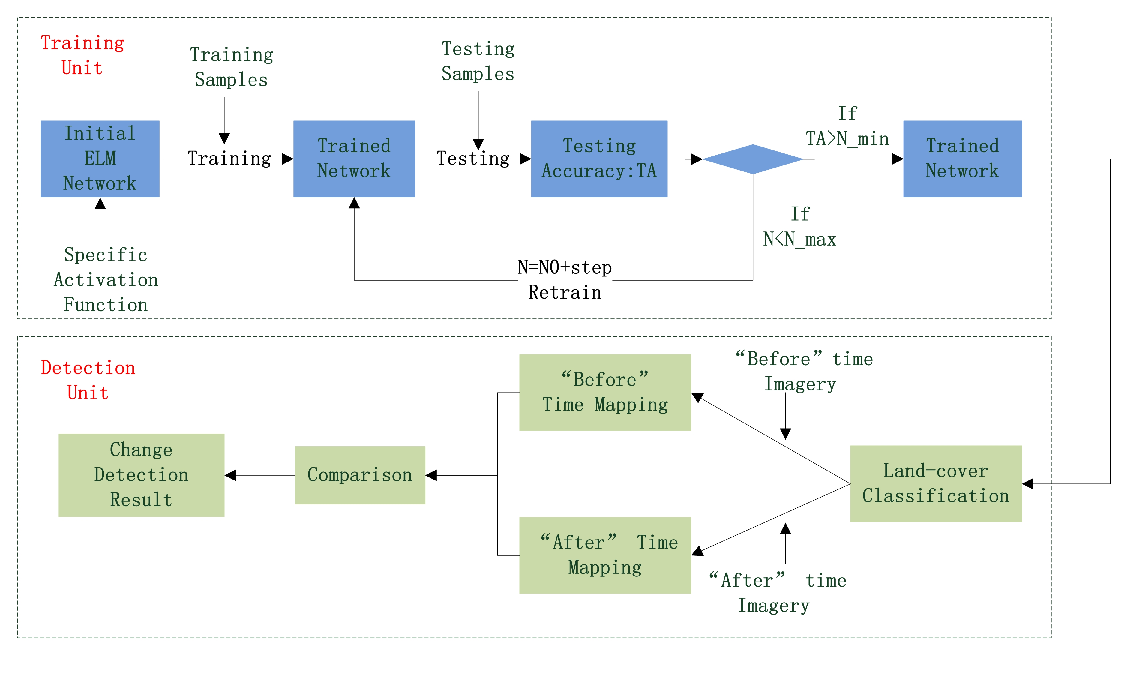
\includegraphics[width=15cm]{method.eps}
\caption{ELM-based Land-cover Change Detection Method}
\label{method}
\end{center}
\end{figure}
\par

\subsubsection{Preparatory Work: Land-cover Categories and Samples}
According to different terrains area and RS imageries, the land-covery can be classified into specific categories. 
In our application, according to the investigation of Taihu Lake region's terrains and the chosen Landsat-7 imageries, we classify the land-cover into five types as described in Table 1.
In order to ensure precision and representative, training and testing samples should be labeled through visual interpretation and field survey\cite{YuXiu-Lan1999}.
\begin{table}[h]
\scriptsize{
\begin{center}
\begin{tabular}[bt]{|c|c|c|}\hline
Ground object category	& Image features	& Ground object description \\ \hline
Urban			& Purple, faint red	& road or building \\ \hline
Water			& Blue or deep blue	&River or pond \\ \hline
Vegetation		& Deep Green, deep Yellow		& Forest,Hill \\ \hline
Arable land		& Green, light green, cyan	& land for agriculture \\ \hline
Wetlands		& Black		& Wetlands \\ \hline
\end{tabular}
\caption{Image Interpretation of Each Ground Object Category}\label{categories}
\end{center}
}
\end{table}
\par
The land-cover category is represented by an integer, ranging from 1 to 5.
Every pixel contains the values of all the bands of the multi-spectral RS imagery.
So every sample can be described as:
$$
\mathbf{x}_i=\left[x_{i1},x_{i2},...,x_{in}  \right]^T \in \mathbf{R}^n  \\
$$
$$
\mathbf{t}_i = f(x) = 
	\begin{cases} 
	1, & \mbox{if type is Urban} \\ 
	2, & \mbox{if type is Water} \\
	3, & \mbox{if type is Vegetation} \\
	4, & \mbox{if type is Arable Land} \\
	5, & \mbox{if type is Wetlands} 
	\end{cases}
$$,
where $\mathbf{x}_i$ is the input, $\mathbf{t}_i$ is the output, $n$ is the number of bands of the RS imagery, i ranges from 1 to $N$, and $N$ is the number of samples.
\par
As the preparatory work of our application and experiments, samples are manually labeled in the RS imagery.
In order to ensure the network's actual availability, both "before" time and "after" sample imageries should contribute to the samples. 
\par

\subsubsection{Training Unit}
Training unit is to build the land-cover classifier for the detection unit.
In the classifier, too few hidden nodes will lead to low classification capability, while too many hidden nodes will cause over-fitting. 
Moreover, the activation function will also greatly influence the classifier's performance.
Therefore, our training unit is responsible for choosing proper hidden node number and activation function.
\par
In training unit, we build the land-cover classification network in the following steps:
\begin{enumerate}[(i)]
\item First, choose a specifice activation function.
\item Second, build the classifier using our land-cover classification network building proceducer, as shown in Algorithm 1.
\item Third, for every activation function, execute the procedure several times and calculate the average testing accuracy.
\item Fourth, choose a proper activation function. It can build a classifier than can achieve the highest average testing accuracy.
\end{enumerate}
\par
In brief, we incrementally training and testing our network with different hidden node number for every activation function. 
The network with the highest average testing accuracy is the one that we build in training unit.
\par
\begin{algorithm}[H]
\caption{Land-cover Classification Network Building Proceducer}
\label{alg1}
\begin{algorithmic}
\REQUIRE Given training sample set $\chi$, testing sample set $\psi$, activation function $g$: 
\STATE Step 1) \textbf{Initialization:} Initialize the land-cover classifier with default hidden node number and $g$
\STATE Step 2) \textbf{Building Step}:
	\WHILE {no enough testing accuracy} 
	\STATE a) increase the hidden node number 
   	\STATE b) training the new network wtih $\chi$
	\STATE c) calculate the network's testing accuracy with set $\psi$
	\IF {the hidden node number is too large}
	\STATE d) record the network with the highest testing accuracy
	\STATE e) break 
	\ENDIF
	\STATE f) record the network with the highest testing accuracy 
	\ENDWHILE
\STATE Step3) return the network with the highest testing accuracy
\end{algorithmic}
\end{algorithm}
\par

\subsubsection{Detection Unit}
Detection unit is mainly responsible for two jobs: calculate the land-cover classification mappings and find the differences between time-series mappings.
\par
Land-cover classification mapping represents the land-cover type of every pixel.
It is drawn through RS imagery classification.
In detail, the procedure contains the following steps.
\begin{enumerate}[(i)]
\item Input the "before" time and "after" time imageries with the size of $N$. $N = W \times H$, where $W$ is the width and $H$ is the height.
\item Preprocess the imagery and translate it into input set: $$\mathbf{x}_i=\left[x_{i1},x_{i2},...,x_{in}  \right]^T \in \mathbf{R}^n$$, where i ranges from $1$ to $N$ and $n$ is the number of bands.
\item Calculate the land-cover type matrix $\mathbf{T}$ using the builded classifier. That is to calculate $\mathbf{T}=\mathbf{H}\beta$, where  
$$\mathbf{H}(\mathbf{w}_1,...,\mathbf{w}_M,b_1,...,b_M,\mathbf{x}_1,...,\mathbf{x}_N) = 
\begin{bmatrix}
g(\mathbf{w}_1 \cdot \mathbf{x}_1 + b_1) & \cdots & g(\mathbf{w}_M \cdot \mathbf{x}_1 + b_M) \\
\vdots & \ddots & \vdots \\
g(\mathbf{w}_1 \cdot \mathbf{x}_N + b_1) & \cdots & g(\mathbf{w}_M \cdot \mathbf{x}_N + b_M)
\end{bmatrix}_{N \times M}, 
$$
$$
\beta = \begin{bmatrix}\beta_i^T \\ \vdots \\ \beta_M^T \end{bmatrix}_{M \times m},  \mathbf{T} = \begin{bmatrix}\mathbf{t}_1^T \\ \vdots \\ \mathbf{t}_N^T \end{bmatrix}_{N \times m}. 
$$
$\mathbf{w}_i$, $\mathbf{b}_i$, $M$ and $\beta_i$ are the paramters of the builded classifier, $m$ is the number of land-cover categories.
\item Translate the vector $\mathbf{t}_i^T$ into land-cover type of every pixel. The position of the largest element in $\mathbf{t}_i^T$ is the integer that represents the land-cover type. 
\item Draw the land-cover classification mapping. Different land-cover type of the pixel use different colour.
\end{enumerate}
\par

Detection unit finds the interesting changes through comparison of land-cover classification mappings.
The comparison mainly contains two aspects.
\begin{enumerate}[(i)]
\item First, every location's land-cover transition can be calculated.
This is done simply by checking the "before" time land-cover type and the "after" time land-cover type of every pixel.
Moreover, the land-cover transition mapping, which represents the land-cover type change of every position, can be drawn.
\item Second, the change of coverage of every land-cover type can be calculated.
Through comparing the coverage area, we can find the expansion or shrinkage of every land-cover type.
For example, the expansion map of urban area can be drawn.
What's more, land-cover classification pie charts can be drawn to accurately and visually display the land-cover change of every type.
\end{enumerate}
\par


%%%%%%%%%%%%%%%%%%%%%%%%%%%%%%%%%%%%%%%%%%%%%%%%%%%%%%%%%%%
%%%%%%%%%%%%%        Evaluation       %%%%%%%%%%%%%%%%%%%%%
%%%%%%%%%%%%%%%%%%%%%%%%%%%%%%%%%%%%%%%%%%%%%%%%%%%%%%%%%%%
\section{Evaluation}\label{benchmarkexperiment}
\subsection{Training Unit Analysis}
Training unit mainly builds the land-cover classifier.
This chapter will analysis the classifier building procedure and its result.
\par
Firstly, we show our original imageries and samples in Figure 2.
The pair of time-series imageries are token by LANDSAT-5 satellite with TM sensor mode.
They both cover Taihu Lake region in east China.
Five labeled $20\times20$ squares of different land-cover types are shown in Figure 2(c).  
\begin{figure}[H]
\centering
\subfigure["Before" time imagery, token on Dec. 25, 2001]{
\label{Fig.sub.1}
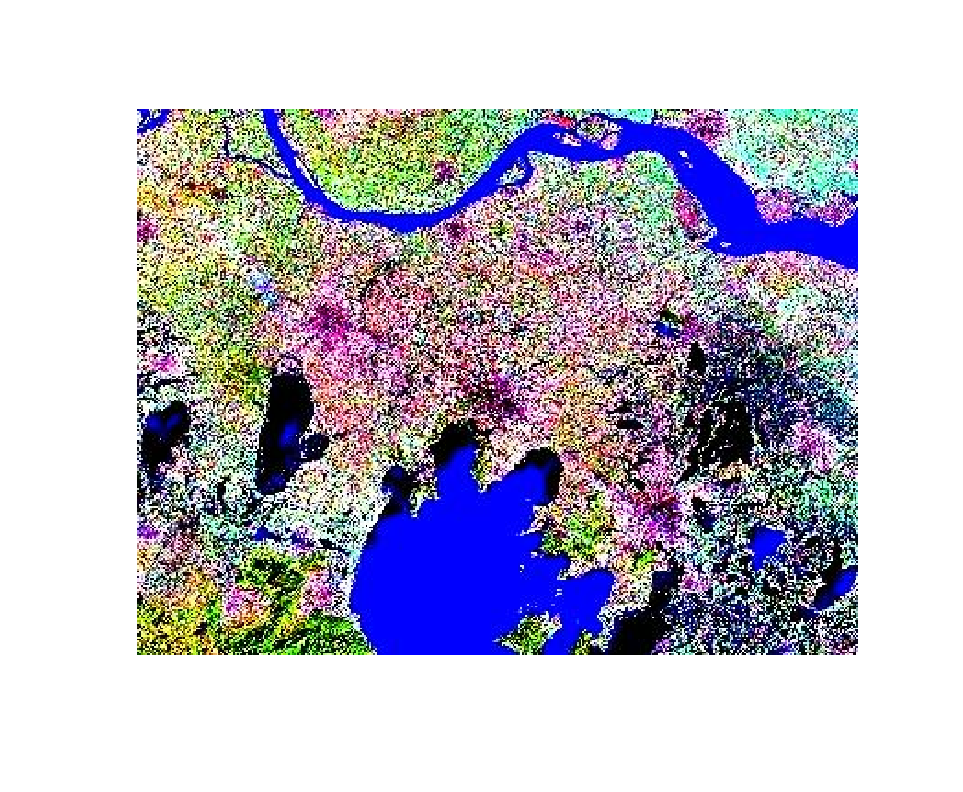
\includegraphics[width=0.45\textwidth]{bi.eps}}
\subfigure["After" time imagery, token on Feb. 28, 2008]{
\label{Fig.sub.2}
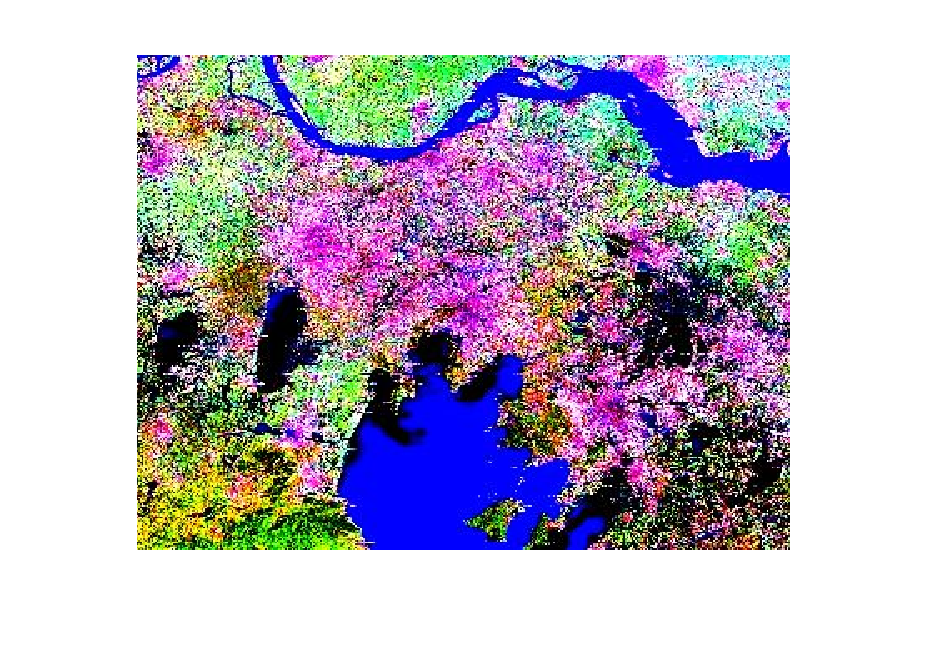
\includegraphics[width=0.45\textwidth]{ai.eps}}
\subfigure[Samples of Different Land-cover Types]{
\label{Fig.sub.2}
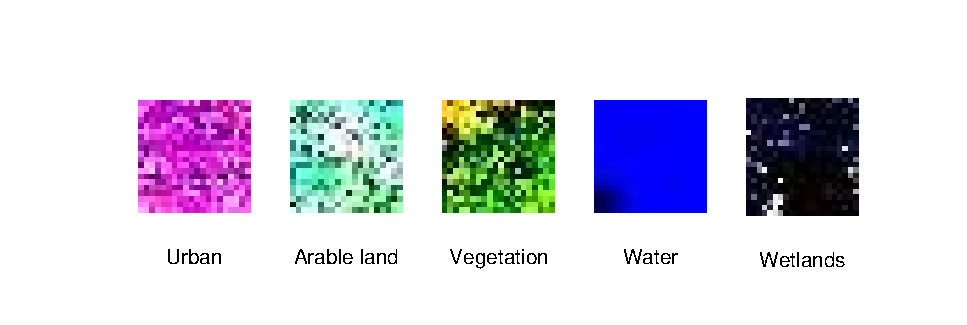
\includegraphics[width=0.8\textwidth]{samples.eps}}
\caption{Original Imageries and Samples}
\label{Fig.lable}
\end{figure}
\par

The land-cover classifier building procedure can be seen in Figure 3.
In Figure 3, the hidden node number increases from 10 to 400 with a step of 3.
Everytime, the network is trained and tested several times and the average testing accuracy is calculated.
\par
From the figure, we can give three conclusions.
\begin{enumerate}[(i)]
\item First, all the activation functions, except for hardlim, performs similarly with different hidden node number.
\item Second, the average testing accuracy improves greatly before the hidden node number reaches 100, but is stabilized when the hidden node number exceeds about 150.
\item Third, the network with 350 to 400 hidden nodes and the activation function of tribas can achieve the testing accuracy of more than 98\%.
 This network can be chosen as the builded land-cover classifier of training unit.  
\end{enumerate}
\begin{figure}[H]
\begin{center}
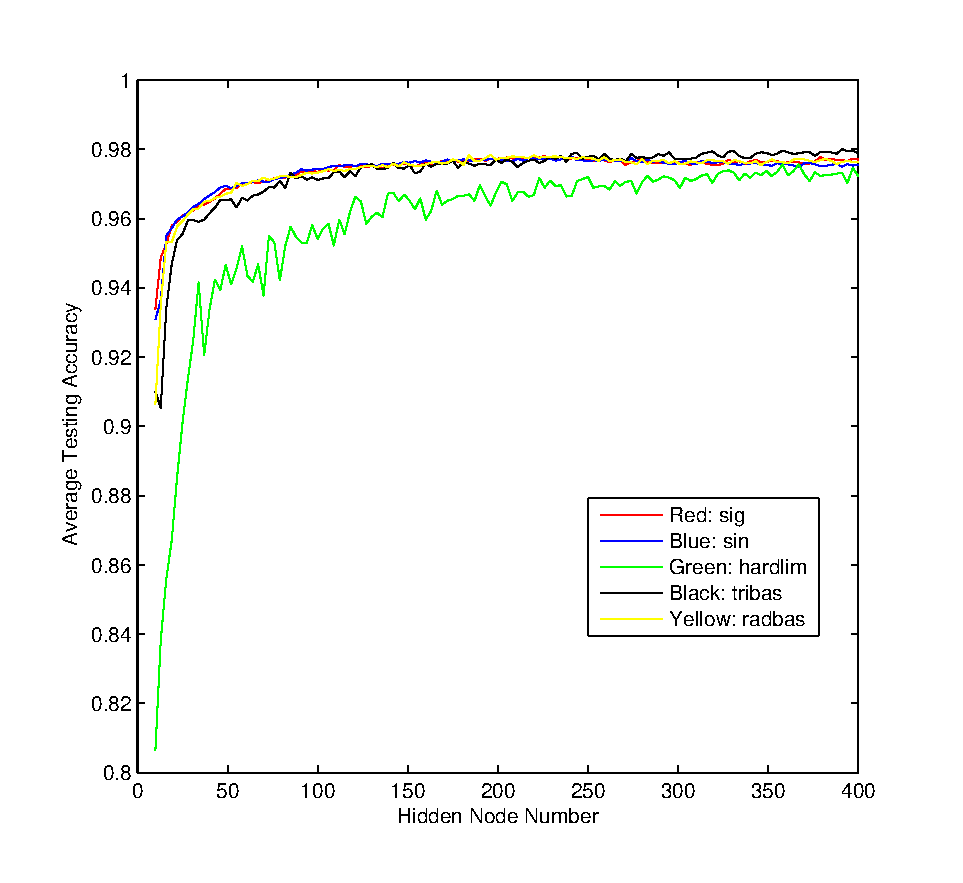
\includegraphics[width=0.8\textwidth]{itr.eps}
\caption{Land-cover Classifier Building Procedure and Result.}
\label{method}
\end{center}
\end{figure}
\par

\subsection{Land-cover Classification Performance of ELM}
This chapter will analysis ELM network's fast training speed and high generalisation performance in RS imagery classification.
Moreover, comparison between ELM and SVM, BP network will be evaluated. 
\par

One factor that we will compare is their training time.
The hidden node number of ELM network is set to 100 and sin is chosen as the activation function.
This ensures testing accuracy to be more than 95\%.
Similarly, both parameters of SVM and BP networks are adjusted to ensure testing accuracy to be more than 95\%.
The average training time of all the tree methods is shown in Figure 4.
\begin{figure}[H]
\begin{center}
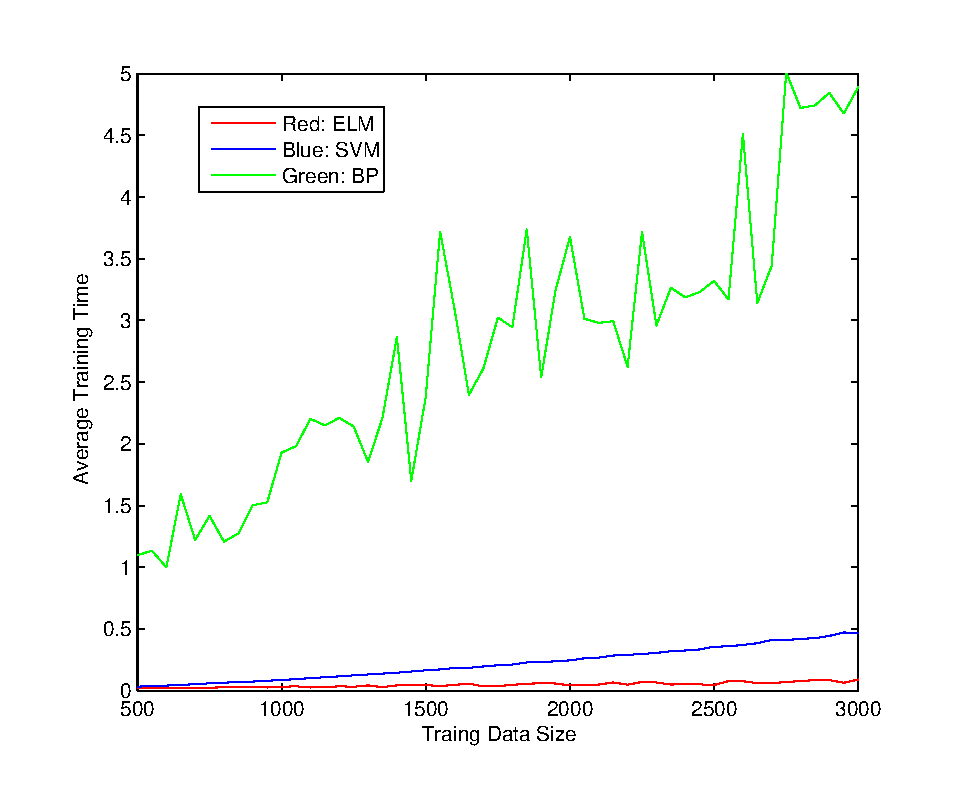
\includegraphics[width=0.8\textwidth]{tt.eps}
\caption{Average Training Time of ELM, BP and SVM. }
\label{method}
\end{center}
\end{figure}
\par

From the figure we can argue that ELM always costs the least training time.
When the data size increases, the training time of BP network increases greatly and are unstable.
While the training time of ELM network increases linearly and the slope is small.
From Figure 4 and Table 2, we can see the BP network takes about 47 times more time than ELM to learn. 
And SVM network takes nearly 7 times more time to learn than ELM.
\par

\begin{table}[h]
\scriptsize{
\begin{center}
\begin{tabular}[bt]{|p{0.5cm}||p{0.93cm}|p{0.93cm}|p{1.14cm}||p{0.93cm}|p{0.93cm}|p{1.14cm}||p{0.93cm}|p{0.93cm}|p{1.14cm}|}\hline

 & \multicolumn{3}{|c||}{ELM} & \multicolumn{3}{|c||}{BP} & \multicolumn{3}{|c|}{SVM} \\ \cline{2-10}
Data Size &Training Time &Testing Time &Testing Acc &Training Time &Testing Time &Testing Acc &Training Time &Testing Time &Testing Acc \\ \hline
500 &0.0180 &0.0060 &97.3200\% &0.0312 &0.0054 &93.4000\% &1.4743 &0.0082 &95.8000\% \\ \hline
750 &0.0270 &0.0060 &97.1333\% &0.0582 &0.0107 &93.6000\% &1.3774 &0.0082 &92.7333\% \\ \hline
1000 &0.0320 &0.0070 &97.1000\% &0.0844 &0.0166 &94.3000\% &1.7887 &0.0083 &93.3300\% \\ \hline
1250 &0.0370 &0.0060 &97.1360\% &0.1170 &0.0239 &94.5600\% &1.7557 &0.0089 &95.7760\% \\ \hline
1500 &0.0480 &0.0120 &97.1733\% &0.1596 &0.0341 &95.1333\% &1.9633 &0.0083 &96.3467\% \\ \hline
1750 &0.0560 &0.0110 &97.1429\% &0.2174 &0.0418 &95.1429\% &2.2055 &0.0085 &95.7943\% \\ \hline
2000 &0.0610 &0.0120 &97.4150\% &0.2471 &0.0518 &95.5000\% &2.3117 &0.0089 &93.9900\% \\ \hline
2250 &0.0590 &0.0140 &97.3422\% &0.3221 &0.0624 &95.1111\% &2.1111 &0.0090 &96.4089\% \\ \hline
2500 &0.0780 &0.0140 &97.5560\% &0.3605 &0.0741 &95.3200\% &2.8407 &0.0088 &96.5120\% \\ \hline
2750 &0.0800 &0.0150 &97.5382\% &0.4165 &0.0876 &95.2000\% &3.3488 &0.0092 &95.9673\% \\ \hline
3000 &0.0840 &0.0150 &97.4500\% &0.4551 &0.0989 &95.2333\% &3.3238 &0.0094 &96.1267\% \\ \hline
\end{tabular}
\caption{RS Imagery Classification Performance Comparision among ELM, BP and SVM.}
\label{specification}
\end{center}
}
\end{table}

The other factor that we will compare is their generalisation performance.
We can evaluate it in the following two aspects.
\begin{enumerate}[(i)]
\item First, the testing accuracy of ELM is always higher than that of BP and SVM networks.
\item Second, ELM network can soon reaches high generalization performance, even with small training data set.
while the other two networks need more training samples to assure high testing accuracy.
\end{enumerate}
\par

In summary, we can argue that ELM network cost much less time to train and can achieve higher generalisation performance than BP and SVM in RS imagery classification.

\subsection{Change Detection Result Analysis}
Two major contributions of detection unit are time-series land-cover classification mappings and land-cover change detection result.
This chapter will evaluate the two contributions.
\par
The time-series land-cover classification mappings are shown in Figure 5. 
Five different colours represent five different land-cover types.
Compared to the original imageries in Figure 2(a)(b), we can visually judge that both mappings truly reflect the actual ground surface.
\par

Coverage change mapping of every land-cover type is one of the formats to display land-cover change detection result.
The cyan area in Figure 6 shows the expansions of urban.
From the mapping, we can visually judge that a lot of urban area has been expanded around the original urban area.
\par

\begin{figure}[H]
\centering
\subfigure["Before" Time]{
\label{Fig.sub.1}
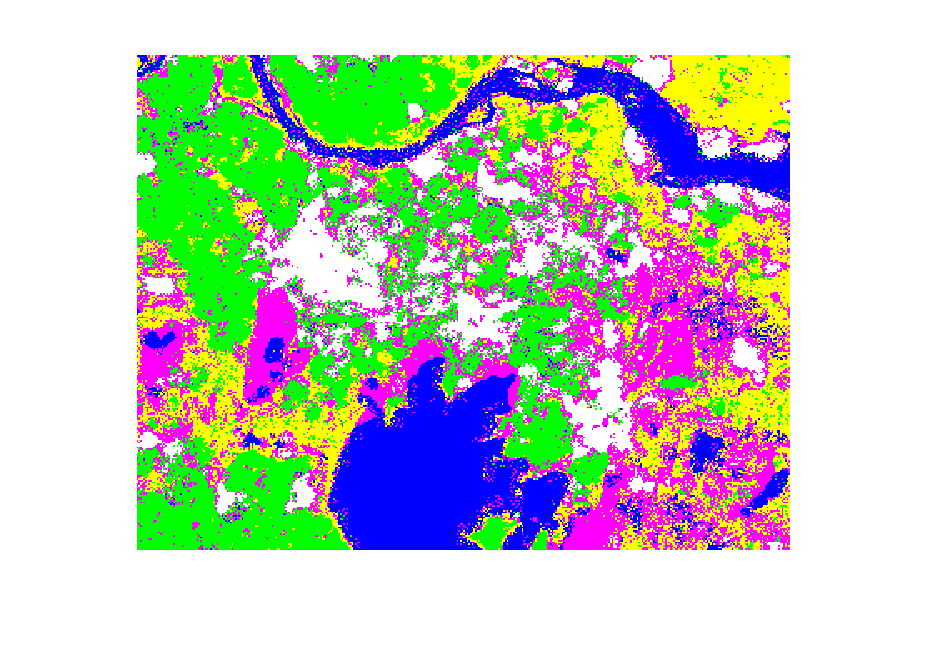
\includegraphics[width=0.4\textwidth]{bc.eps}}
\subfigure["After" Time]{
\label{Fig.sub.2}
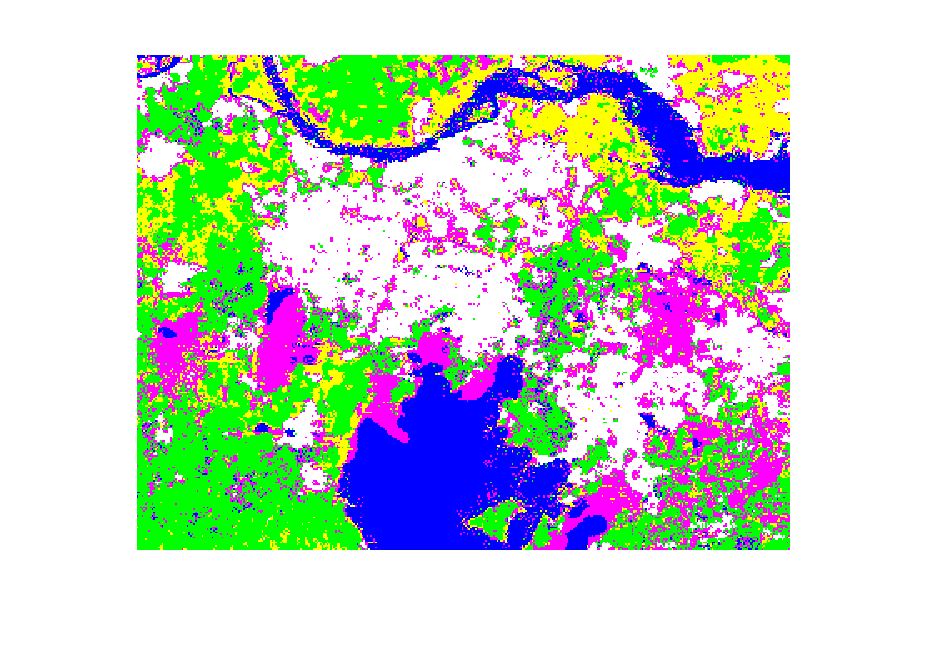
\includegraphics[width=0.4\textwidth]{ac.eps}}
\caption{Time-series Land-cover Classification Mappings. Whrite area represents urban, blue area represents water, yellow area represents arable land, green area represents vegetation, manenta area represents wetlands.}
\label{Fig.lable}
\end{figure}

\begin{figure}[H]
\begin{center}
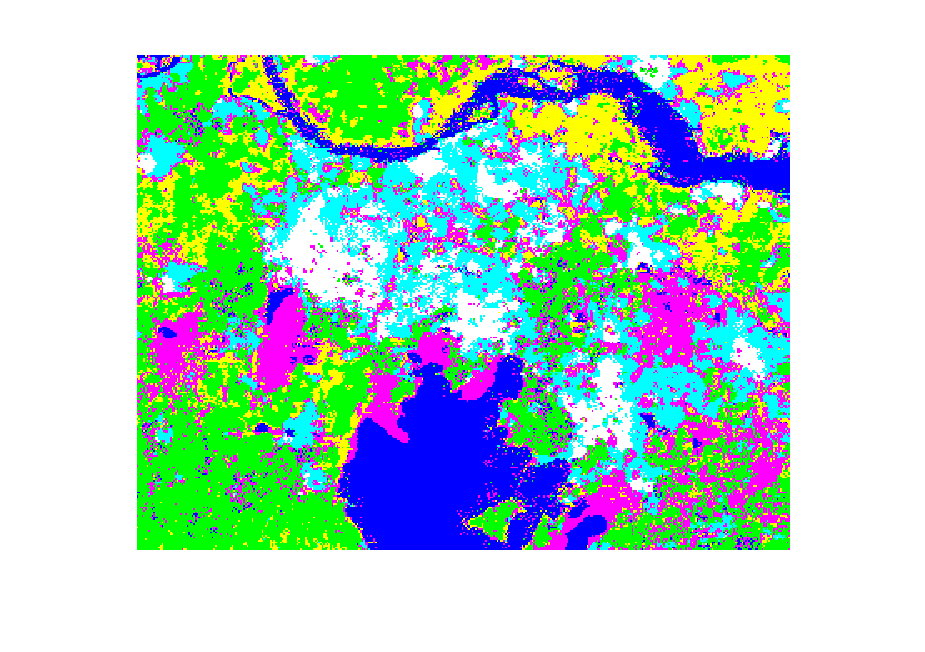
\includegraphics[width=0.8\textwidth]{dr.eps}
\caption{Urban Area Change Detection. The cyan are the new urban area that appears in year 2008, compared to the land-cover of year 2001.}
\label{method}
\end{center}
\end{figure}
\par

Another format to display land-cover change is the proportion pie chart and histogram, as shown in Figure 7 and Figure 8.
In both Figure 7 and Figure 8, the proportion of every land-cover type is displayed and compared.
From the result, we can easily conclude that the urban area is rapidly expanding, from $13\%$ to $24\%$.
While the area of water, arable land and wetlands is shrinking.
\par
\begin{figure}[H]
\centering
\subfigure["Before" Time]{
\label{Fig.sub.1}
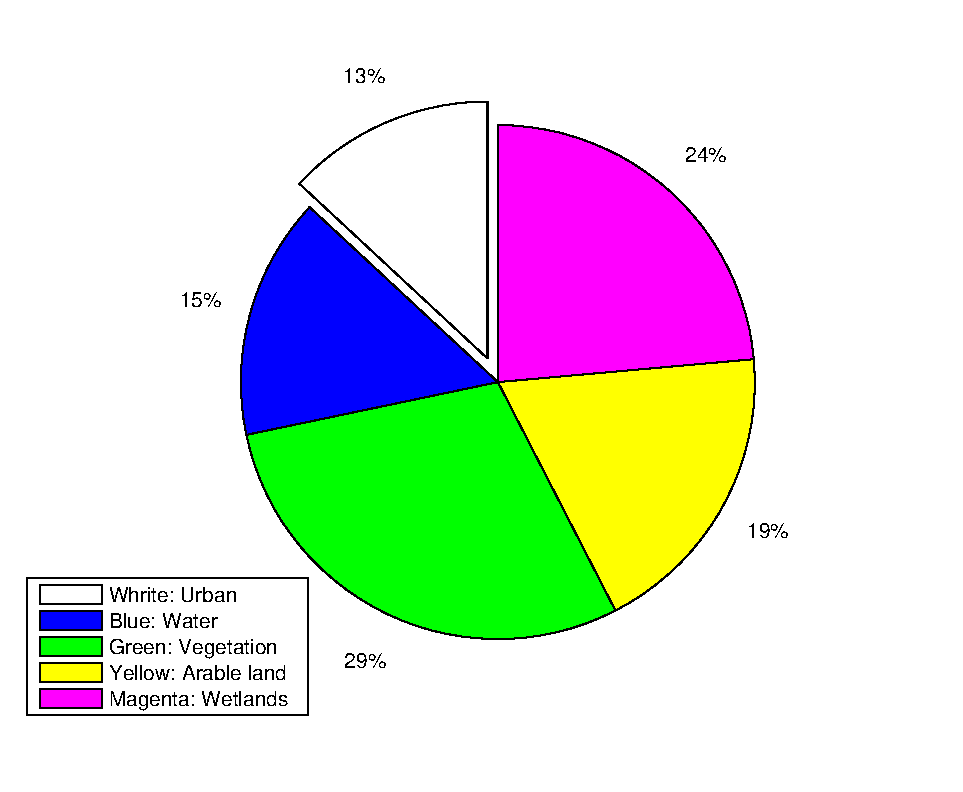
\includegraphics[width=0.4\textwidth]{bc2.eps}}
\subfigure["After" Time]{
\label{Fig.sub.2}
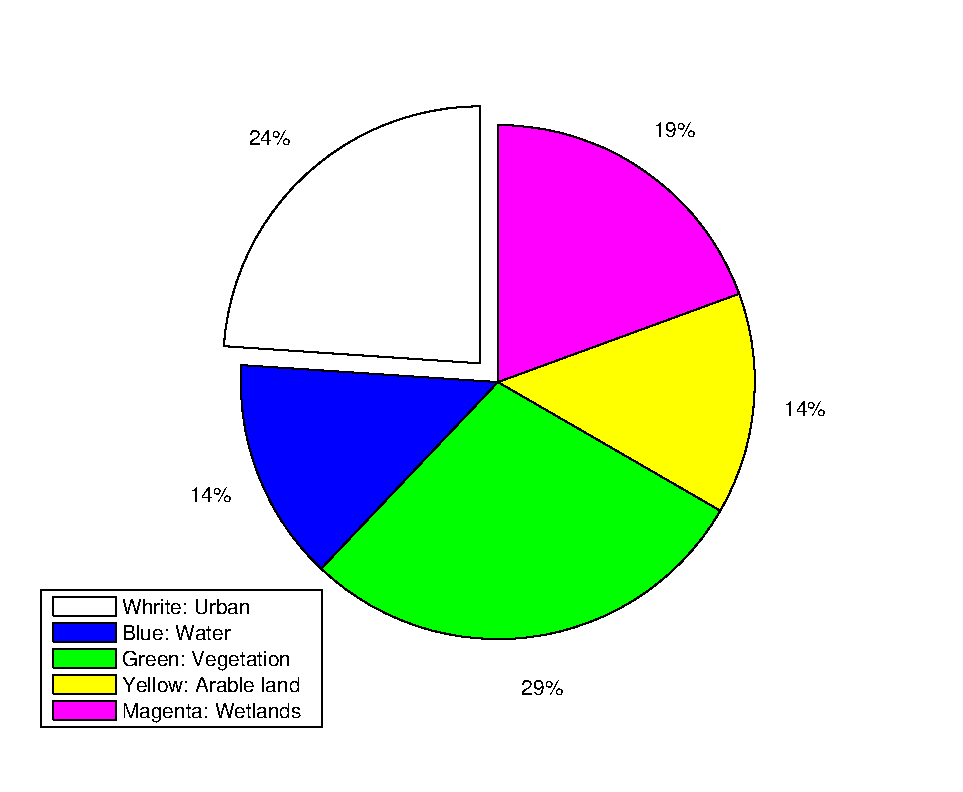
\includegraphics[width=0.4\textwidth]{ac2.eps}}
\caption{Land-cover Classification Result}
\label{Fig.lable}
\end{figure}

\begin{figure}[H]
\begin{center}
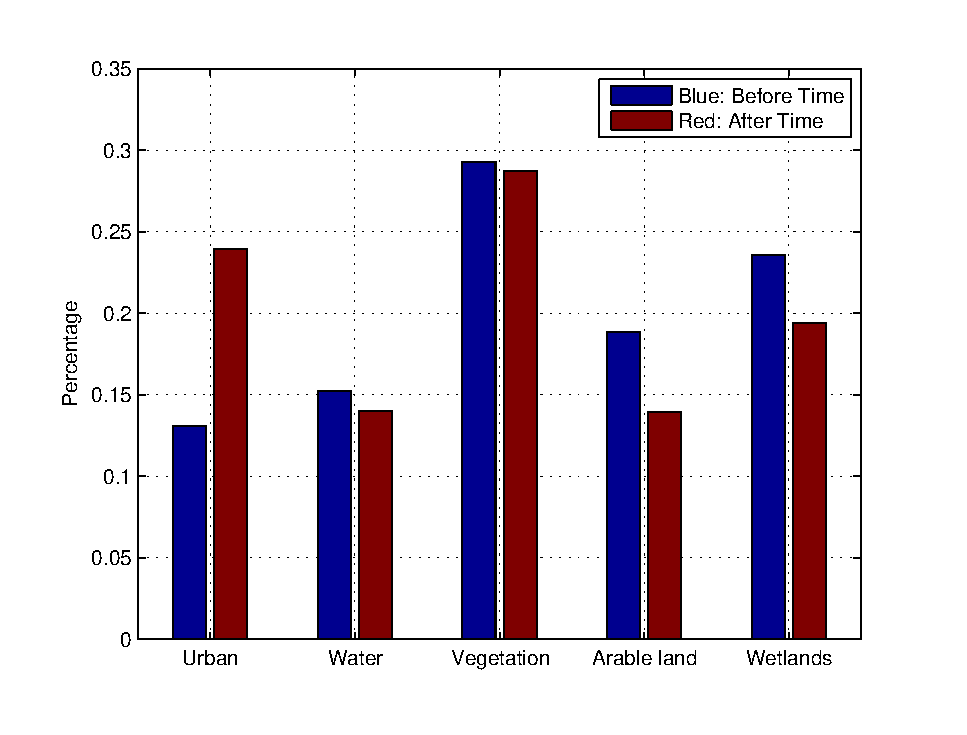
\includegraphics[width=0.8\textwidth]{dr2.eps}
\caption{Change Detection Result of Five Different Land-cover Area .}
\label{method}
\end{center}
\end{figure}
\par
 

%%%%%%%%%%%%%%%%%%%%%%%%%%%%%%%%%%%%%%%%%%%%%%%%%%%%%%%%%%%
%%%%%%%%%%%%%        Discussion       %%%%%%%%%%%%%%%%%%%%%
%%%%%%%%%%%%%%%%%%%%%%%%%%%%%%%%%%%%%%%%%%%%%%%%%%%%%%%%%%%
\section{Discussion}
This paper proposes an ELM-based land-ocver change detection method with high accuracy, high efficiency and less human intervention.
It is the first application of applying ELM to time-series RS imagery processing.
The application result and comparison experiments prove that ELM can be sucessfully applied in RS imagery classification.
\par

Our ELM-based land-cover change detection method is shown in Figure 1.
It mainly contains the training unit and the detection unit.
The training unit is to build the land-cover classifier.
Through the analysis of Figure 3, we can find that the testing accuracy of our builded network can achieve more than 97\%.
This characteristic means that the classifier can be applied in the detection unit for the classification of other RS imageries.
Detection unit will draw the land-cover classification mapping.
And then calculate the land-cover change through comparison of time-series land-cover classification mappings.
\par

Our method sucessfully analysis land usage change of Taihu Lake region from the year 2001 to the year 2008.
The urban area expansion mapping is shown in Figure 6.
Compared to the original time-series imageries in Figure 2(a)(b), Figure 6 accurately reflects the expansion of urban area. 
The proportion pie chart and histogram in Figure 7 and Figure 8 provide more statistic results of change detection.
The result proves that ELM can be sucessfully applied in time-series RS imagery processing.
\par 

In order to highlight ELM's advantages in RS imageries classification, the paper evaluate the comparison experiments between ELM network and SVM,BP network.
According to the training time comparison results in Figure 4 and Table 2, we can directly conclude that ELM network costs much less train time than SVM and BP network.
Moreover, the train time of ELM network increases linearly and slowly when the training data size increases.
From the average testing accuracy statistics in Table 2, we can find that ELM's testing accuracy is always higher than SVM and BP network.
For example, when the training and testing data size reaches 3,000, the testing accuracy of ELM exceedes 97\%, while SVM and BP network only reach about 96\% and 95\%.
\par

%%%%%%%%%%%%%%%%%%%%%%%%%%%%%%%%%%%%%%%%%%%%%%%%%%%%%%%%%%%
%%%%%%%%%%%%%        Future Work and Conclusion  %%%%%%%%%%
%%%%%%%%%%%%%%%%%%%%%%%%%%%%%%%%%%%%%%%%%%%%%%%%%%%%%%%%%%%
\section{Future Work and Conclusion}
More research topics of large scale time-series RS imagery processing with ELM have been proposed in our research group.
Our future work is to expand the land-cover change detection method to parallel computing on hadoop-based cloud infrastructure.
At the same time, ELM will be applied to other RS imagery applications, such as object identification, rainfall estimation, cloud cover evaluation and so on.
What's more, ELM's capability of online learning, such as OS-ELM, will be explored.
we consider it a good resolution to the training of large scale and increasing RS imageries. 
\par

Time-series RS imagery processing plays a more and more important role in various fields.
But the new problems, such as increasing satellite data, are challenging the traditional methods.
This paper contributes the first application of ELM network to time-series RS imagery processing.
It proposes an ELM-based land-cover change detection method with less human intervention, higher processing efficincy and higher detection accuracy.
Using this method, the land-cover change of Taihu Lake region from the year 2001 to the year 2008 is accurately detected.
The result evaluation proves that ELM can be sucessfully applied in time-series RS imagery processing.
Moreover, our comparison experiments show that ELM outperforms SVM and BP network in terms of training time and testing accuracy, when applied in RS imagery classification.
\par

%%%%%%%%%%%%%%%%%%%%%%%%%%%%%%%%%%%%%%%%%%%%%%%%%%%%%%%%%%%
%%%%%%%%%%%%%        Acknowledgement             %%%%%%%%%%
%%%%%%%%%%%%%%%%%%%%%%%%%%%%%%%%%%%%%%%%%%%%%%%%%%%%%%%%%%%
\section{Acknowledgement}
This work is funded in part by China 973 subprograms
NO. 2003CB316906 and NO. 2003CB317006; China NSF
programs NO. NSFC60503018, No. 60525202, and No.
60533040; and National Key Technology R&D Program No.
2006BAH02A01.
\par
\bibliography{/home/jychen/Documents/MachineLearning/mypaper/paper/reference}

\end{document} 
